%           ******************************************************
%          **   course         : Advanced Computer Architecture  **
%         ***   HomeWork       : 03                              ***
%        ****   Topic          : Simulation on gem5              ****
%        ****   AUTHOR         : Reza Adinepour                  ****
%         ***   Student ID:    : 402131055                       ***
%          **   Github         : github.com/rezaAdinepour/       **
%           ******************************************************

\documentclass[12pt]{exam}

\usepackage{setspace}
\usepackage{listings}
\usepackage{graphicx,subfigure,wrapfig}
\usepackage{multirow}
\usepackage{blindtext}
\usepackage{multicol}
\setlength{\columnsep}{1cm}
\usepackage{hyperref}
\hypersetup{
	colorlinks=true,
	linkcolor=blue,
	filecolor=magenta,      
	urlcolor=cyan,
	pdftitle={Overleaf Example},
	pdfpagemode=FullScreen,
}
\usepackage{xcolor, soul}
\usepackage{code-style}
\usepackage{caption}

\usepackage{algorithm}
\usepackage{algpseudocode}


\DeclareCaptionFont{white}{\color{white}}
\DeclareCaptionFormat{listing}{%
	\parbox{\textwidth}{\colorbox{gray}{\parbox{\textwidth}{#1#2#3}}\vskip-4pt}}
\captionsetup[lstlisting]{format=listing,labelfont=white,textfont=white}
\lstset{frame=lrb,xleftmargin=\fboxsep,xrightmargin=-\fboxsep}


\usepackage[margin=20mm]{geometry}
\usepackage{xepersian}
\settextfont{XB Niloofar}

\newcommand{\class}{درس معماری کامپیوتر پیشرفته}
\newcommand{\term}{نیم‌سال اول ۰۲-۰۳}
\newcommand{\college}{دانشکده مهندسی کامپیوتر}
\newcommand{\prof}{استاد: دکتر فربه}

\singlespacing
\parindent 0ex

\lstset{
keywordstyle=\textbf,
identifierstyle=, 
stringstyle=\ttfamily,
commentstyle=\color{LimeGreen}, 
stringstyle=\ttfamily,
numberstyle=\footnotesize,
showstringspaces=false} 
\begin{document}


% -------------------------------------------------------
%  Thesis Information
% -------------------------------------------------------

\newcommand{\ThesisType}
{سمینار}  % پایان‌نامه / رساله
\newcommand{\ThesisDegree}
{کارشناسی ارشد گرایش معماری کامپیوتر}  % کارشناسی / کارشناسی ارشد / دکتری
\newcommand{\ThesisMajor}
{مهندسی کامپیوتر}  % مهندسی کامپیوتر
\newcommand{\ThesisTitle}
{تمرین شبیه‌سازی سری ۲}
\newcommand{\ThesisAuthor}
{\href{https://github.com/rezaAdinepour/M.Sc-AUT/tree/main/Advanced Computer Architecture}{\textcolor{black}{رضا آدینه پور}} - ۴۰۲۱۳۱۰۵۵}
\newcommand{\ThesisSupervisor}
{جناب آقای دکتر فربه}
\newcommand{\ThesisDate}
{۱۰ آبان ۱۴۰۲}
\newcommand{\ThesisDepartment}
{دانشکده مهندسی کامپیوتر}
%\newcommand{\ThesisUniversity}
%{دانشگاه صنعتی امیرکبیر}

% -------------------------------------------------------
%  English Information
% -------------------------------------------------------

%\newcommand{\EnglishThesisTitle}{A Standard Template for Course Exercise}


\pagestyle{empty}

\begin{center}


\includegraphics[scale=0.2]{images/logo.png}

%\vspace{0.5cm}
%\ThesisUniversity \\[-0.3em]
\vspace{0.3cm}
\large\ThesisDepartment\\

\begin{large}
\vspace{0.5cm}


%\ThesisMajor

\end{large}

\vspace{1.5cm}

{عنوان:}\\[1.2em]
{\LARGE\textbf{\ThesisTitle}}\\ 
\vspace{1cm}
%\begin{latin}
%{\Large\textbf\EnglishThesisTitle}
%\end{latin}

\vspace{2cm}

{نگارش}\\[.5em]
{\large\textbf{\ThesisAuthor}}

\vspace{1.5cm}

{استاد راهنما}\\[.5em]
{\large\textbf{\ThesisSupervisor}}

\vspace{1cm}



\vspace{2cm}

\ThesisDate

\end{center}

\newpage


% These commands set up the running header on the top of the exam pages
\pagestyle{head}
\firstpageheader{}{}{}
\runningheader{صفحه \thepage\ از \numpages}{}{\class}
\runningheadrule
\vspace{0pt}


\textbf{\textcolor{blue}{• سوال اول}} \\ 
دو شبه کد زیر را برای مسئله ضرب ماتریس‌ها در نظر بگیرید و گام‌های زیر را با توجه به آن کامل کنید.\\

• الگوریتم اول:
\begin{latin}
\begin{algorithm}
	\caption{Matrix multiplication}\label{alg1:cap}
	\begin{algorithmic}
		\Require Input Matrix A and B
		\Require Let C be a new matrix of the appropriate size
		\For{i from 1 to n:}
			\For{j from 1 to p:}
			\State $sum \gets 0$
				\For{k from 1 to m:}
					\State $sum \gets A_{ik}\times B_{kj}$
				\EndFor
			\EndFor
		\EndFor
		\State $return \ C$
	\end{algorithmic}
\end{algorithm}
\end{latin}

• الگوریتم دوم:
\begin{latin}
	\begin{algorithm}
		\caption{Matrix multiplication}\label{alg2:cap}
		\begin{algorithmic}
			\Require Input Matrix A and B
			\Require Let C be a new matrix of the appropriate size
			\Require Pick a tile size $T = \Theta (\sqrt{M})$
			\For{I from 1 to n:}
				\For{J from 1 to p:}
					\For{K from 1 to m:}
						\State $A_{I:I+T, K:K+T} \times B_{K:K+T, J:J+T} \times C_{I:I+T, J:J+T}$
						\For{i from I to min(I+T, n)}
							\For{j from J to min(J+T, p)}
								\State $sum \gets 0$
							\EndFor
							\For{k from K to min(K+T, m)}
								\State $sum \gets sum + A_{ik} \times B_{kj}$
							\EndFor
							\State $C_{ij} \gets C_{ij} + sum$
						\EndFor
					\EndFor
				\EndFor
			\EndFor
			\State $return \ C$
		\end{algorithmic}
	\end{algorithm}
\end{latin}





\textbf{• گام اول: }\\
شبه کد های آورده شده را به کد \texttt{Python} یا \texttt{C++} تبدیل کرده و آن‌ها را کامپایل و فایل کامپایل شده را بر روی یک سیستم ساده فاقد حافظه نهان در شبیه‌ساز \texttt{Gem5} اجرا کنید. برای درک بهتر تفاوت ها و هدف این تمرین، نیاز است ماتریس‌هایی با بیش از ۱۰۰ سطر و ستون تعریف کنید. مقادیر مربط به درایه‌های ماتریس‌ها را با تابع \texttt{Rand} تولید کنید. برای این گام باید کد‌های مربوطه و تصاویر اجرای کد‌ها بر روی \texttt{Gem5} و نیز فایل \texttt{stats} تولید شده را درقالب یک فایل زیپ با نام \texttt{step1} در فایل نهایی پاسخ خود قرار دهید.

\textbf{• راهنمای گام اول: }\\
برای اجرای کد بر روی شبیه‌ساز از دستور زیر استفاده می‌شود:

\begin{latin}
	\texttt{build/X86/‫‪gem5.opt‬‬[‫‪path of the config file][‫‪path of your compiled code]}
\end{latin}

برای پیکربندی شبیه‌ساز به صورت یک سیستم فاقد حافظه نهان، باید فایل \texttt{config} مربوطه را اجرا کنید. آموزش نحوه کدنویسی و ایجاد این فایل در آدرس زیر، \href{https://www.gem5.org/documentation/learning_gem5/part1/simple_config/}{\textcolor{magenta}{اینجا}} موجود است.

شما می‌توانید درصورت تمایل، توضیحات را مطالعه و کد‌های این فایل را بررسی کنید. در غیر این صورت می‌توانید از فایل آماده آن که در مسیر \texttt{configs/learning\_gem5/part1/simple.py}
وجود دارد استفاده کنید.






\textbf{• گام دوم: }\\
فایل \texttt{stats} مربوط به کد‌ها را بررسی کرده و پارامتر‌های زیر را برای دو کد پیدا کرده و در گزارش خود بیاورید. فایل \texttt{stats} را می‌توانید در مسیر \texttt{gem5/m5out} پیدا کنید.
\begin{latin}
	\begin{itemize}
		\item IPC
		\item Number of busy cycles
	\end{itemize}
\end{latin}







\textbf{• گام دوم: }\\
در این گام باید کد‌های مربوط به دو شبه‌کد را بر روی یک سیستم دارای دو سطح حافظه نهان  L1 و L2 اجرا کنید. برای این گام مد پردازنده را CPU Simple Timing درنظر بگیرید. Associativity حافظه نهان لایه اول داده و دستور‌العمل را ۴ و حافظه نهان لایه دوم را ۸ و نیز اندازه هر بلاک را ۶۴ درنظر بگیرید. سایز حافظه نهان لایه اول و دوم اختیاری است. اما باید در گزارش ذکر شود. باید تصاویر اجرای کدها بر روی \texttt{gem5} و نیز فایل \texttt{stats} تولید شده را در قالب یک فایل \texttt{Zip} با نام \texttt{step2} در فایل نهایی پاسخ خود قرار دهید.
\begin{latin}
	\begin{itemize}
		\item IPC
		\item Number of busy cycles
		\item L1i cache hit and miss rate
		\item L1d cache hit and miss rate
		\item L2 cache hit and miss rate
	\end{itemize}
\end{latin}

\textbf{• راهنمای گام اول: }\\
برای اینکه \texttt{gem5} را به‌صورت یک سیستم دارای حافظه نهان پیکربندی کنید، از فایل \texttt{config} موجود در مسیر

\texttt{configs/deprecated/example/se.py} استفاده کنید. این فایل به شما اجازه می‌دهد که حافظه نهان L1 و L2 را تعریف کنید و سایز هرکدام و نیز \texttt{Associativity} آن‌ها و دیگر پارامتر‌های مرتبط را تعریف و مقدار‌دهی کنید. می‌توانید از دستورات زیر برای این منظور استفاده کنید:

\begin{latin}
	\begin{itemize}
		\item \texttt{--cpu-type={TimingSimpleCPU||DerivO3CPU||MinorCPU}}
		\item \texttt{--cache $\rightarrow$ enable L1 cache.}
		\item \texttt{--L2cache $\rightarrow$ enable L2 cache.}
		\item \texttt{--L1d\_size = Size}
		\item \texttt{--L1i\_size = Size}
		\item \texttt{--L2\_size = Size}
		\item \texttt{--L1d\_assoc = Associativity}
		\item \texttt{--L1i\_assoc = Associativity}
		\item \texttt{--L2\_assoc = Associativity}
		\item \texttt{--cacheline\_size = cache line (block) size}
	\end{itemize}
\end{latin}
 
 
 
 
 
 
 
 
 
 
\textbf{• گام چهارم: }\\
فایل \texttt{stats} مربوط به کد‌ها را بررسی کرده و پارامتر‌های زیر را برای دو کد پیدا کرده و در گزارش ارسالی خود بیاورید.
\begin{latin}
	\begin{itemize}
		\item IPC
		\item Number of busy cycles
		\item L1i cache hit and miss rate
		\item L1d cache hit and miss rate
		\item L2 cache hit and miss rate
	\end{itemize}
\end{latin}





\textbf{• گام پنجم: }\\
در این گام ابتدا اختلاف مقادیر بدست آمده در گام دوم و چهارم را مقایسه کنید و در ادامه علت اختلاف مقادیر پارامتر‌های گام چهارم برای دو شبه‌کد را تحلیل کنید. (درواقع باید تفاوت عملکرد دو کد را بررسی و تاثیر آن بر رفتار سیستم را بیان کنید) \\ \\ \\ \\








\textbf{\textcolor{blue}{• سوال دوم}} \\ 
در پوشه تمرین یک برنامه با نام \texttt{sample.c} قرار دارد که یک لیست پیوندی با اندازه ۱۰۰۰۰ ایجاد کرده و سپس با استفاده از یک تابع بازگشتی، لیست ایجاد شده را معکوس می‌کند. این برنامه را در \texttt{gem5} و با حالت \texttt{se} اجرا کنید و گام‌های زیر را کامل کنید:



\textbf{• گام اول: }\\
در دو نوع پردازنده Cpu Simple Atomic و DerivO3CPU پارامتر‌های IPC و Second Sim را گزارش کنید و دلیل تفاوت در مقدار این پارامتر‌ها برای دو نوع پردازنده را ذکر کنید.



\textbf{• گام دوم: }\\
سعی کنید تابع مورد استفاده به منظور معکوس کردن لیست پیوندی را به شکلی تغییر دهید که عملکرد سیستم را از نظر پارامتر IPC بهبود دهد. با ذکر دلیل مشخص کنید که در کدام نوع پردازنده بهبود بیشتری می‌توان ایجاد کرد؟ \\ \\ \\ \\









\textbf{\textcolor{blue}{• سوال سوم}} \\ 
بررسی کنید که سه Mode مربوط به سیستم حافظه یعنی mode Timing و mode Atomic و mode Functional چه تفاوتی دارند و هرکدام برای چه منظور در شبیه‌سازی استفاده می‌شوند؟ همچنین فایل \texttt{config} استفاده شده در گام اول سوال اول را بررسی کرده و مقادیر پارامتر‌های زیر را در گزارش خود بیاورید.

\begin{itemize}
	\item فرکانس کلاک
	\item مد شبیه‌ساز حافظه
	\item سایز حافظه
\end{itemize}


%\baselineskip = 9mm





\begin{multicols}{1}
	[
	\section{پاسخ سوال اول}
	در این قسمت به بررسی نتایج بدست آمده در سوال اول می‌پردازیم. همچنین شما می‌توانید کد‌های نوشته شده در این بخش را در \href{google.com}{\textcolor{magenta}{اینجا}} یا در انتهای گزارش در «\textcolor{magenta}{\ref{پیوست آ}}» مشاهده کنید. در هر دو کد،‌ ماتریس A را $150\times150$ و ماتریس B را $150\times200$ تعریف کردیم.
	]
	
	\subsection{گام اول}
	\subsubsection{شبه‌کد اول (پایتون)}
	در مرحله اول ابتدا کد پابتون را تست می‌کنیم. برای انجام این مرحله ابتدا باید فایل با پسوند \texttt{.py} را به فایل \texttt{execute} تبدیل کنیم. برای انجام این کار ابتدا با دستور زیر کتابخانه مورد نیاز برای انجام این کار را نصب میکنیم:
	\begin{latin}
		\texttt{pip install pyinstaller}
	\end{latin}
	
	
	پس از نصب کتابخانه با دستور زیر می‌توان فایل \texttt{execute} را تولید کرد:
	\begin{latin}
		\texttt{pyinstaller --onefile [your file name]}
	\end{latin}
	
	حالا فابل \texttt{config} مورد نیاز با شبیه‌سازی خودمان را می‌سازیم.
	از دایرکتوری زیر
	\begin{latin}
		\texttt{gem5/configs/learning\_gem5/part1}
	\end{latin}
	 فایل \texttt{sample.py} را باز کرده و در قسمت
	 \begin{latin}
	 	\texttt{binary = os.path.join()}
	 \end{latin}
	 
	  مسیر فایل \texttt{execute} خود را وارد می‌کنیم.
	  
	  \begin{center}
	  	\begin{figure}[H]
	  		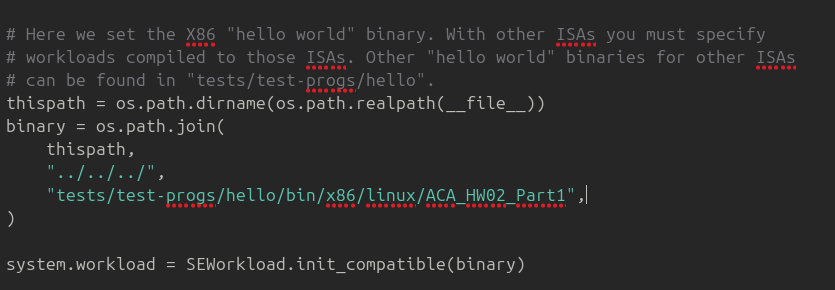
\includegraphics[scale=0.29]{images/img1.png}
	  		\caption{تغییر مسیر فایل کامپایل شده \texttt{Python}}
	  		\label{تغییر مسیر}
	  	\end{figure}
	  \end{center}
	  
	  سپس با دستور زیر شبیه‌سازی را اجرا می‌کنیم:
	  \begin{latin}
	  	\texttt{build/X86/‫‪gem5.opt‬‬ configs/}\\
	  	\texttt{learning\_gem5/part1/simple.py}
	  \end{latin}
	  
	  پس ار تکمیل فرایند شبی‌سازی که قدری زمان‌بر بود خروجی به صورت زیر است:
	  \begin{center}
	  	\begin{figure}[H]
	  		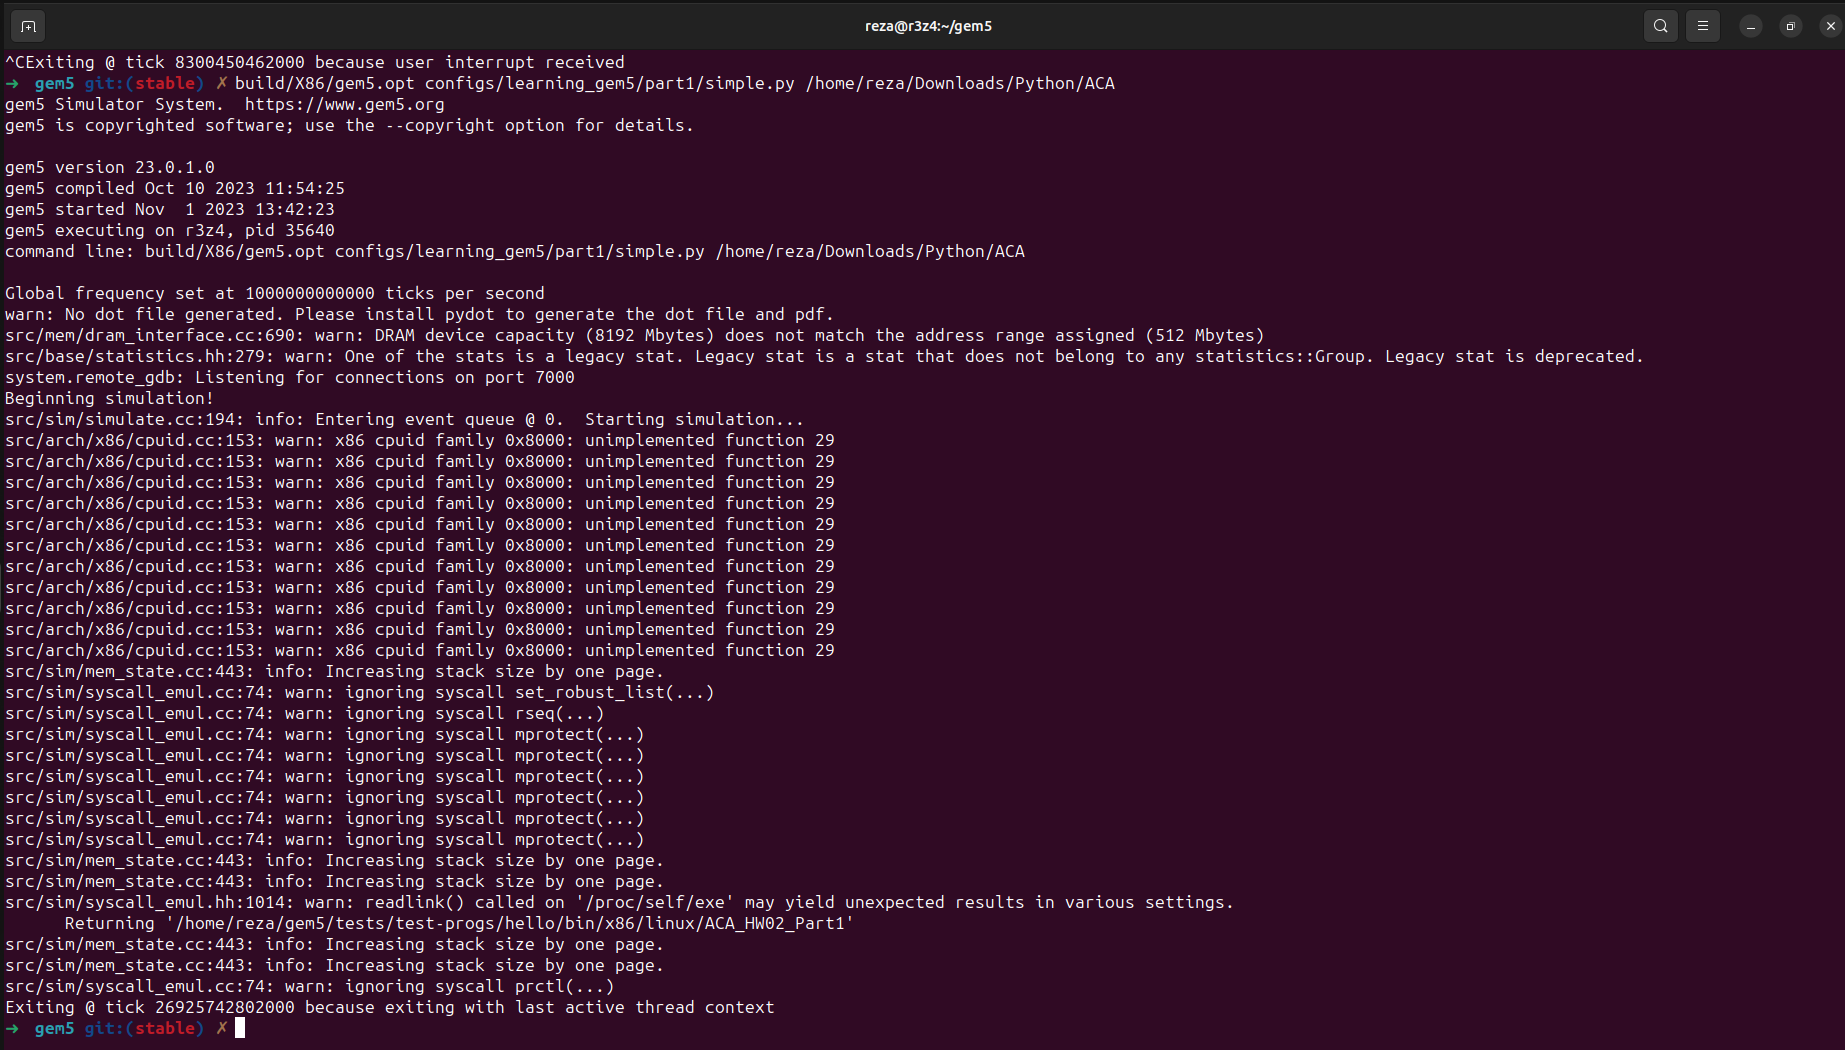
\includegraphics[scale=0.13]{images/img2.png}
	  		\caption{خروجی شبیه‌سازی اول با \texttt{Python}}
	  		\label{خروجی شبیه‌سازی اول با پایتون}
	  	\end{figure}
	  \end{center}
	  
	  متاسفانه شبیه‌سازی با فایل \texttt{python} به‌درستی کار نکرد و نتوانستم مشکل آن‌را پیدا کنم. پس ادامه شبیه‌سازی ها را با کد \texttt{\hl{C++}} انجام می‌دهیم.
	  
	  
	  \subsubsection{شبه‌کد اول (C++)}
	  مشابه با کد پایتون، در فایل \texttt{config} مسیر فایل کامپایل شده \texttt{C++} را می دهیم.
	  \begin{center}
	  	\begin{figure}[H]
	  		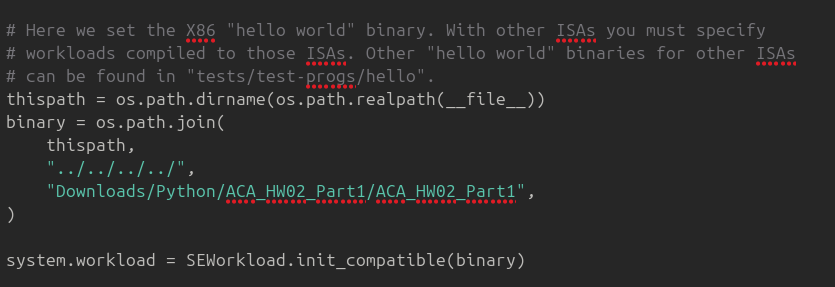
\includegraphics[scale=0.29]{images/img3.png}
	  		\caption{تغییر مسیر فایل کامپایل شده \texttt{C++}}
	  		\label{تغییر مسیر فایل کامپایل شده cpp}
	  	\end{figure}
	  \end{center}
	  
	  خروجی شبیه‌ساز برای شبه‌کد اول \texttt{C++} به صورت زیر است:
	  \begin{center}
	  	\begin{figure}[H]
	  		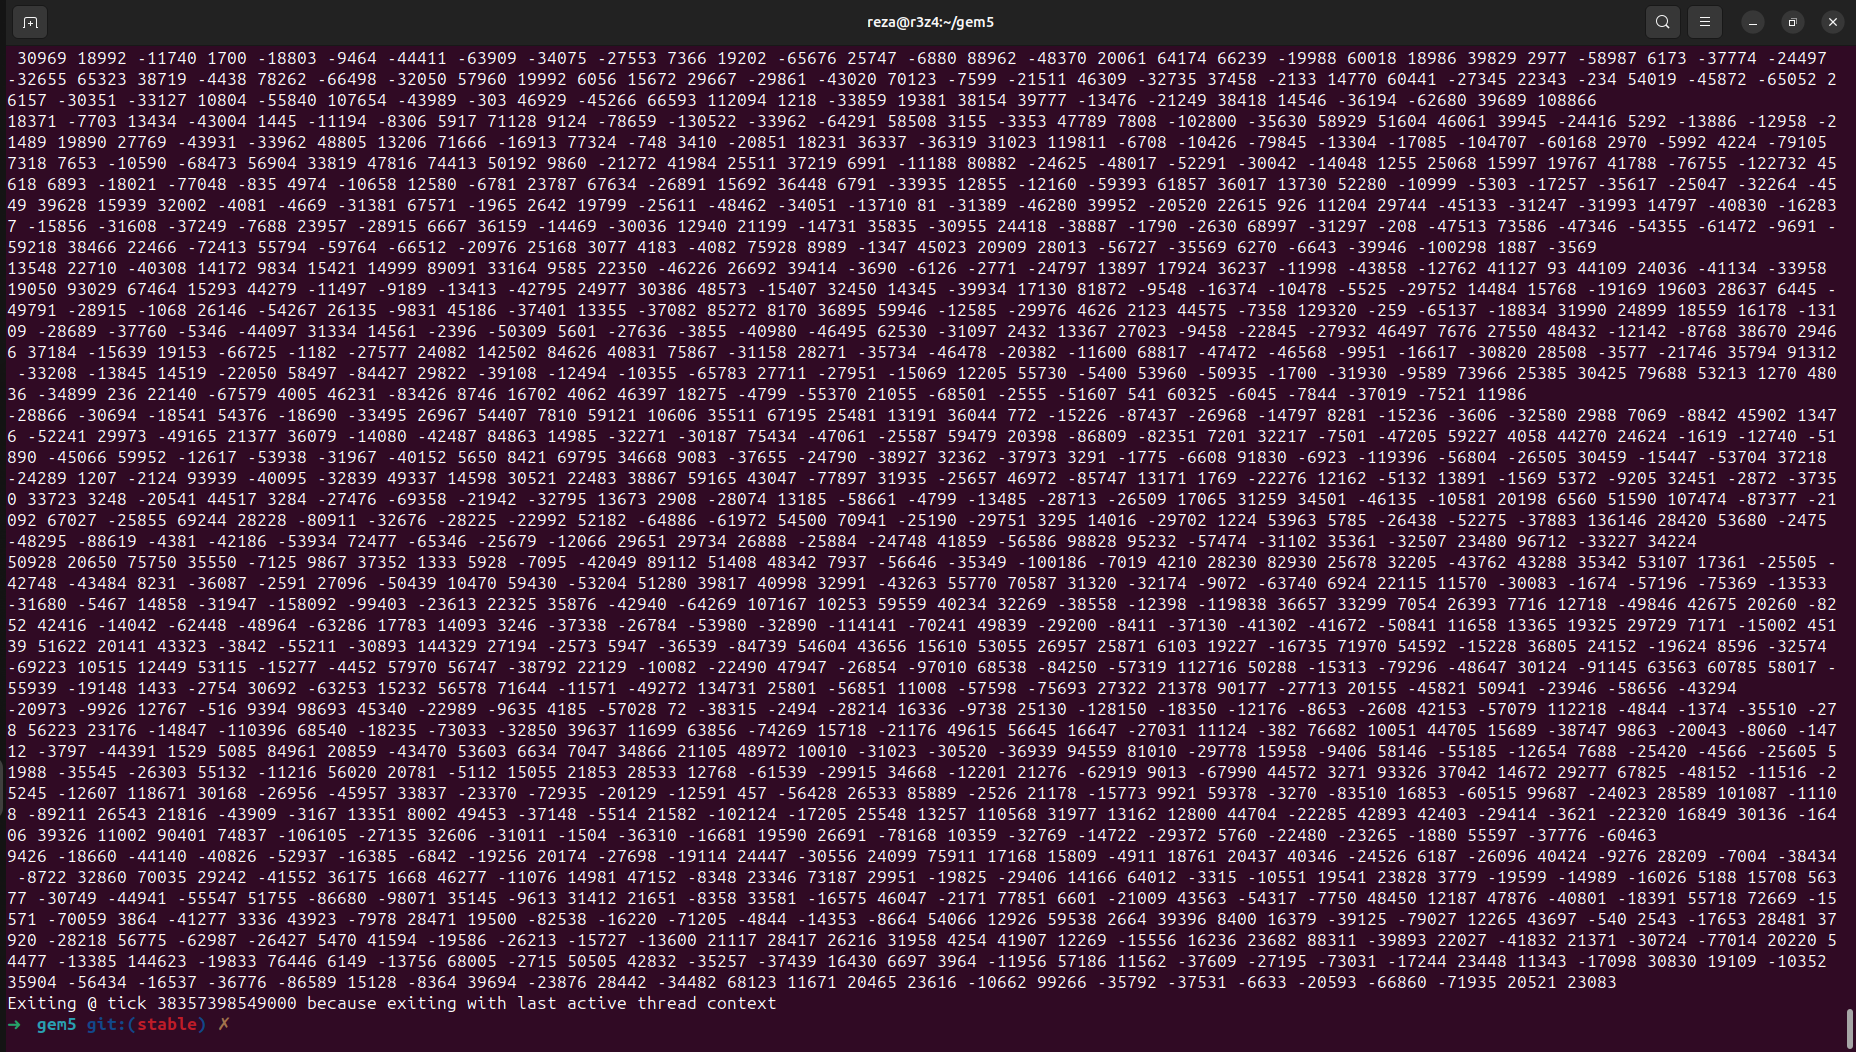
\includegraphics[scale=0.12]{images/img4.png}
	  		\caption{خروجی شبیه‌سازی اول با \texttt{C++}}
	  		\label{خروجی شبیه‌سازی اول با cpp}
	  	\end{figure}
	  \end{center}
	  
	  
	  
	  \subsubsection{شبه‌کد دوم (C++)}
	  برای شبه‌کد دوم، صرفا کد \texttt{‌C++} آن را تست می‌کنیم. مسیر فایل را در فایل ‌\texttt{config} تنظیم می‌کنیم.
	  
	  \begin{center}
	  	\begin{figure}[H]
	  		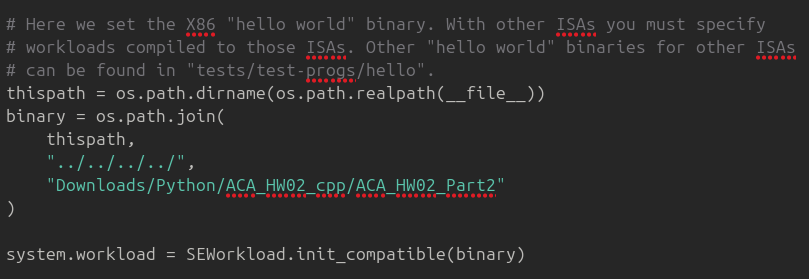
\includegraphics[scale=0.29]{images/img5.png}
	  		\caption{تغییر مسیر فایل کامپایل شده \texttt{C++}}
	  		\label{تغییر مسیر فایل کامپایل شده cpp شبه‌کد دوم}
	  	\end{figure}
	  \end{center}
	  
	   سپس شبیه‌سازی را اجرا می‌کنیم:
	   \begin{center}
	   	\begin{figure}[H]
	   		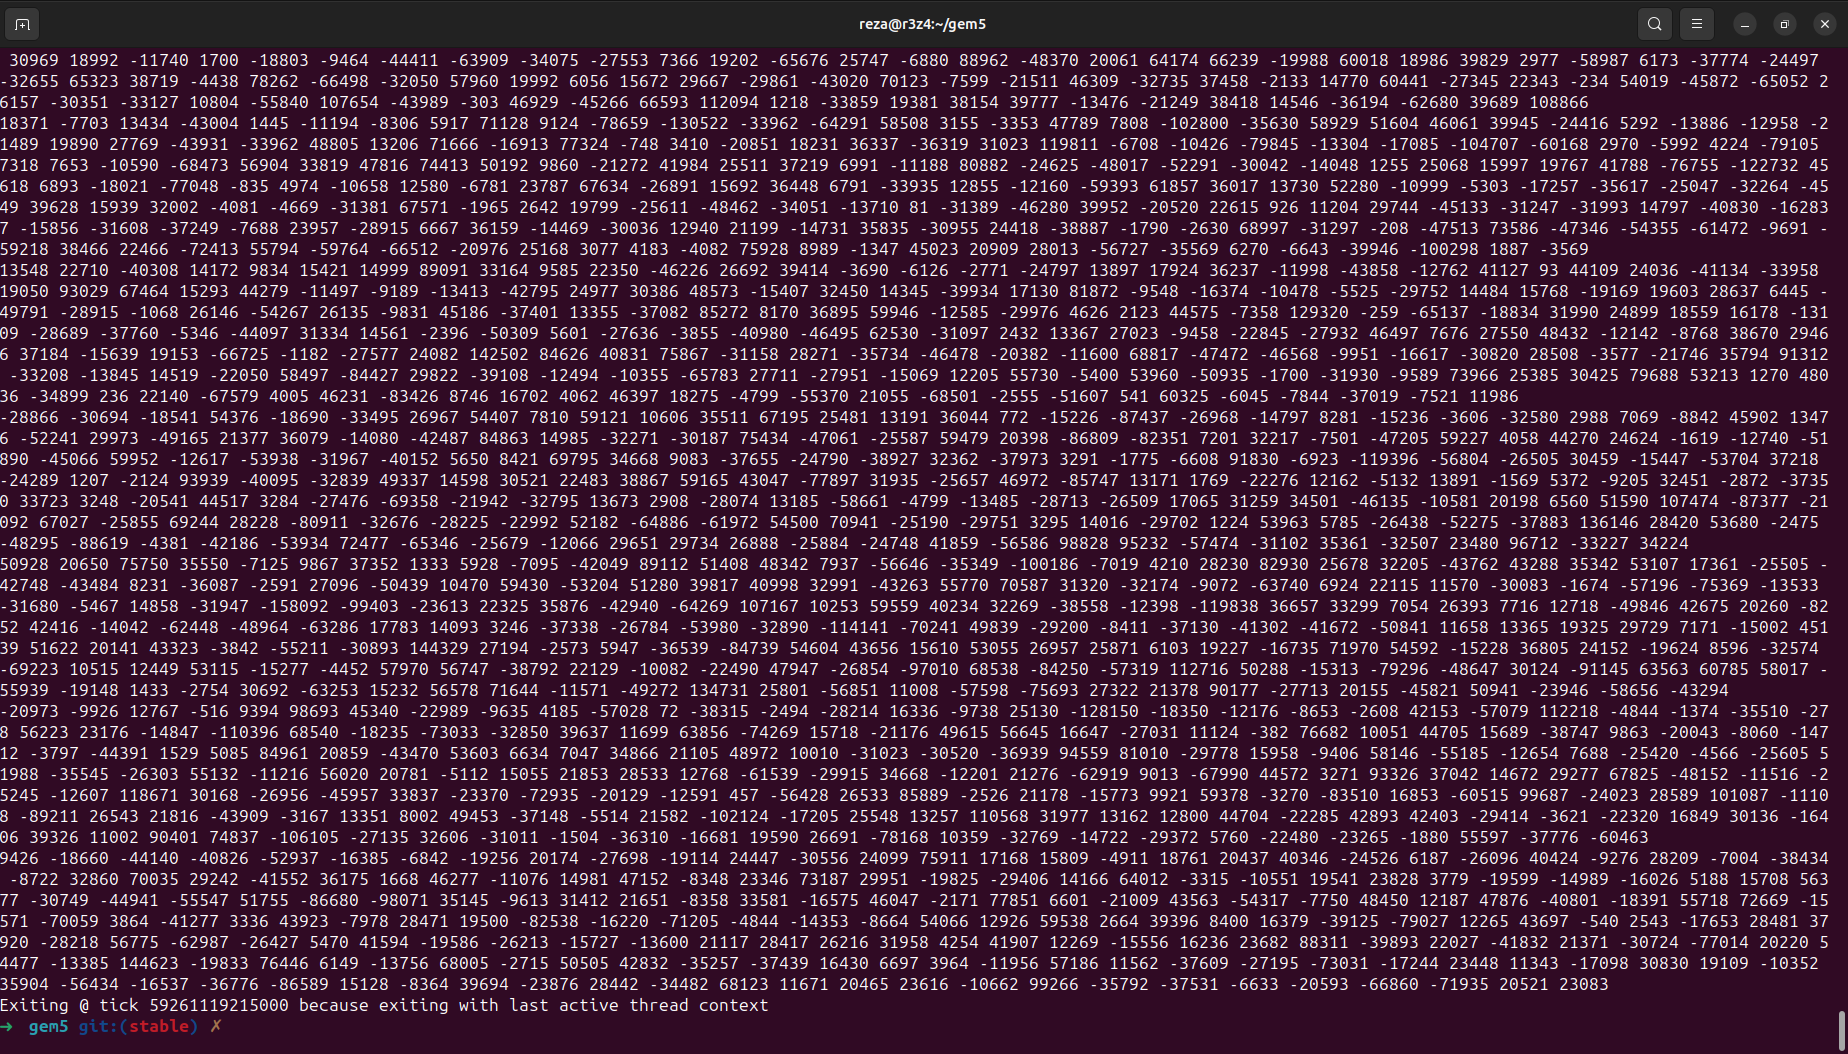
\includegraphics[scale=0.12]{images/img6.png}
	   		\caption{خروجی شبیه‌سازی دوم با \texttt{C++}}
	   		\label{خروجی شبیه‌سازی دوم با cpp}
	   	\end{figure}
	   \end{center}
	  
	  
	  
	  
	  
	  
	  \subsection{گام دوم}
	  \subsubsection{شبه‌کد اول (Python)}
	  در گام بعدی به سراغ فایل \texttt{stats} می‌رویم و پارامتر‌های خواسته شده را گزارش می‌کنیم.
	  \begin{latin}
	  	\begin{itemize}
	  		\item IPC
	  		\item Number of busy cycles
	  	\end{itemize}
	  \end{latin}
	  
	  
	  
	  \subsubsection{شبه‌کد اول (C++)}
	  پارامتر‌های خواسته شده برای کد \texttt{C++} به صورت زیر است:
	  \begin{latin}
	  	\begin{itemize}
	  		\item IPC = 0.011162 $\frac{count}{cycle}$
		  		\item Number of busy cycles: 38357398548.999001
	  	\end{itemize}
	  \end{latin}
	  
	  \subsubsection{شبه‌کد دوم (C++)}
	  پارامتر‌های خواسته شده برای کد \texttt{C++} به صورت زیر است:
	  \begin{latin}
	  	\begin{itemize}
	  		\item IPC = 0.009821 $\frac{count}{cycle}$
	  		\item Number of busy cycles: 59261119214.999001
	  	\end{itemize}
	  \end{latin}
	  
	  
	  
	  
	  
	  
	  
	  
	  \subsection{گام سوم}
	  
	  فایل کانفیگ \texttt{two\_level.py} را از \href{https://github.com/gem5/gem5/blob/stable/configs/learning_gem5/part1/two_level.py}{\textcolor{magenta}{اینجا}} دانلود کردیم و از این فایل به عنوان فایل کانفیگ برای این بخش استفاده می‌کنیم.
	  
	   مسیر فایل کامپایل شده را به صورت زیر در فایل \texttt{two\_level.py} تغییر می‌دهیم:
	  \begin{center}
	  	\begin{figure}[H]
	  		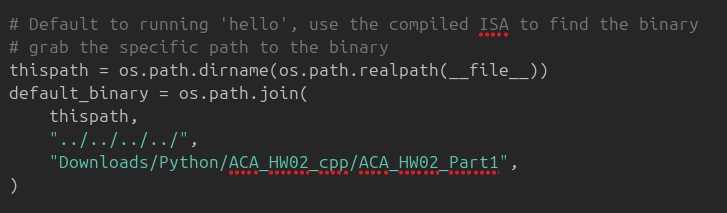
\includegraphics[scale=0.35]{images/img8.png}
	  		\caption{تغییر مسیر فایل کد \texttt{C++} کامپایل شده}
	  		\label{تغییر مسیر فایل}
	  	\end{figure}
	  \end{center}
	  
	  \subsubsection{شبیه‌سازی شبه‌کد اول}
	  با دستور زیر، شبه‌کد اول را شبیه‌سازی می‌کنیم:
	  
	  \begin{latin}
	  	\texttt{build/X86/gem5.opt configs/}
	  	
	  	\texttt{learning\_gem5/part1/two\_level.py}
	  	
	  	\texttt{--l1d\_size=128kB --l1i\_size=64kB}
	  	
	  	\texttt{--l2\_size=1MB}
	  \end{latin}
	  
	  در این بخش سایز Cache L1 را ۶۴ کیلوبایت و سایز Cache L2 را ۱ مگابایت درنظر گرفتیم.
	  
	  خروجی شبیه‌سازی به صورت زیر است:
	  \begin{center}
	  	\begin{figure}[H]
	  		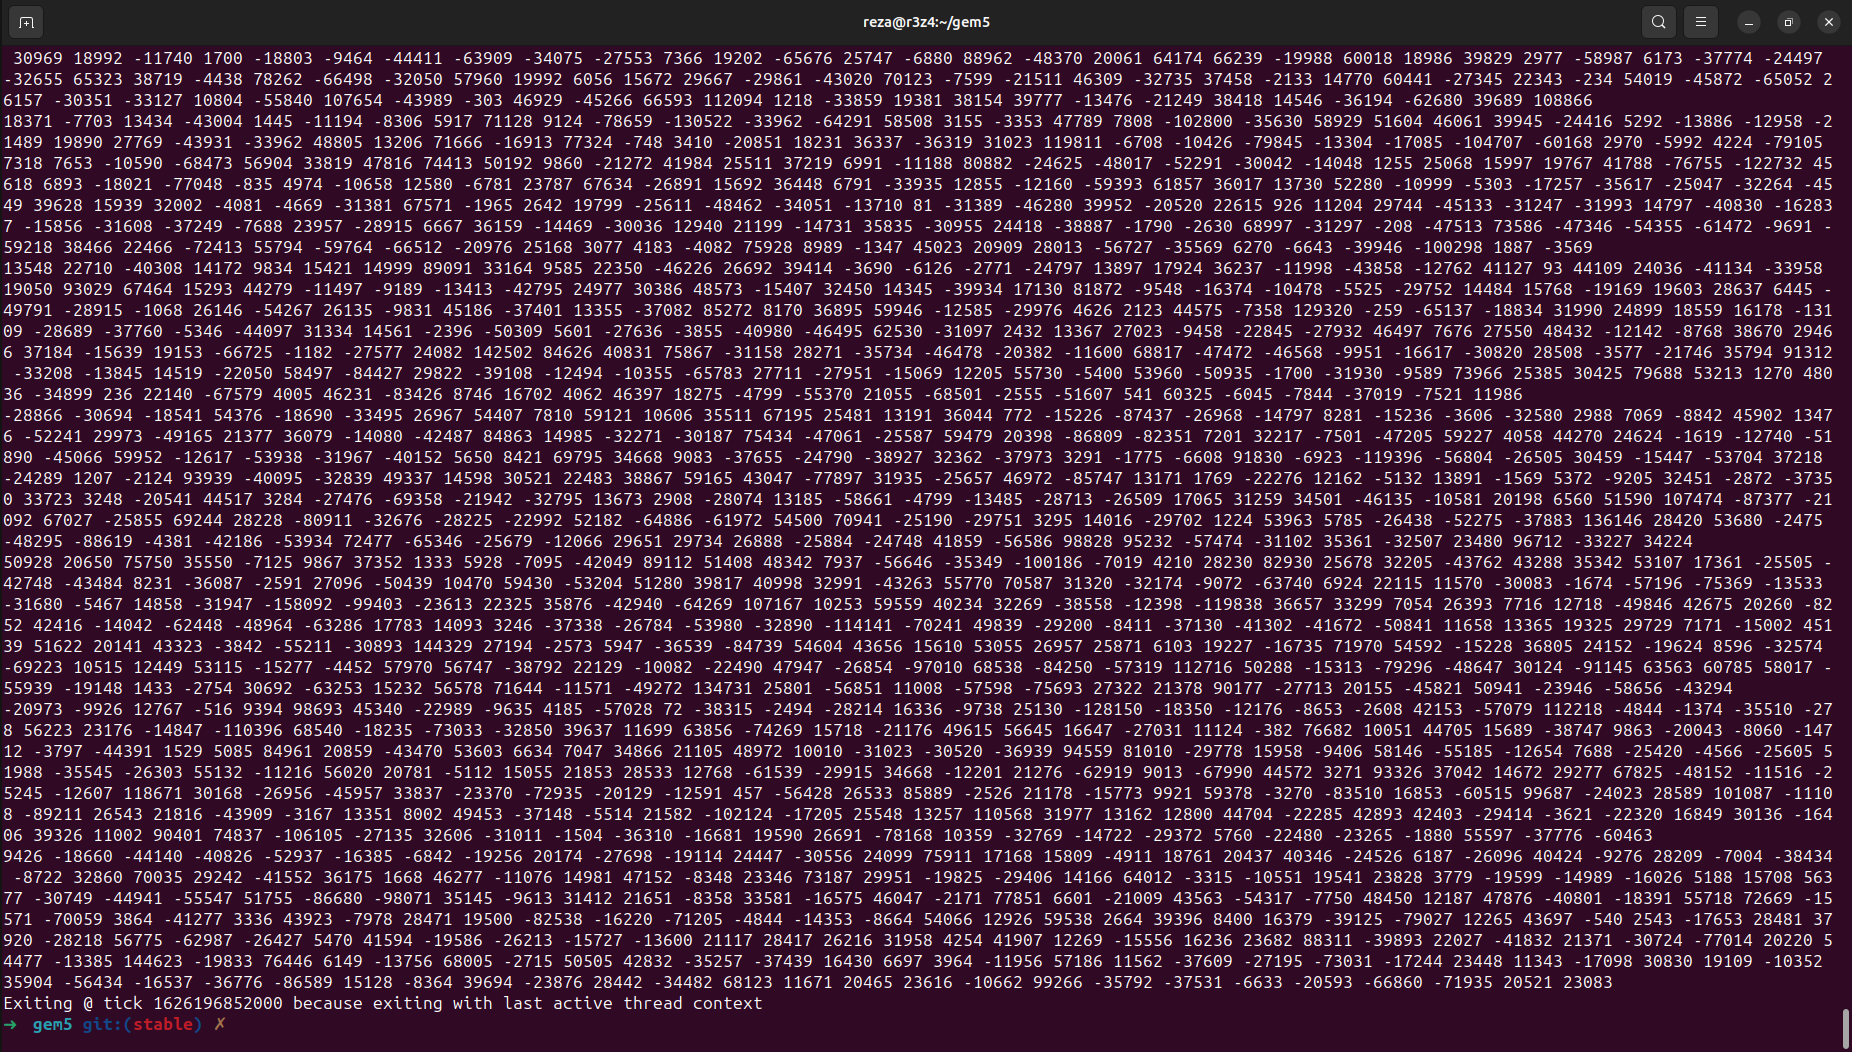
\includegraphics[scale=0.12]{images/img9.png}
	  		\caption{خروجی شبیه‌سازی شبه‌کد اول}
	  		\label{خروجی شبیه‌سازی شبه‌کد اول}
	  	\end{figure}
	  \end{center}
	  
	  
	  
	
	
	\subsubsection{شبیه‌سازی شبه‌کد دوم}
	مسیر فایل کامپایل شده را در فایل کانفیگ تغییر داده و با دستور زیر کد را شبیه‌سازی می‌کنیم:
	سایز \texttt{Cache} ها همان مقدار قسمت قبل هستند.
	\begin{latin}
		\texttt{build/X86/gem5.opt configs/}
		
		\texttt{learning\_gem5/part1/two\_level.py}
		
		\texttt{--l1d\_size=128kB --l1i\_size=64kB}
		
		\texttt{--l2\_size=1MB}
	\end{latin}
	
	
	 خروجی شبیه‌سازی به صورت زیر است:
	\begin{center}
		\begin{figure}[H]
			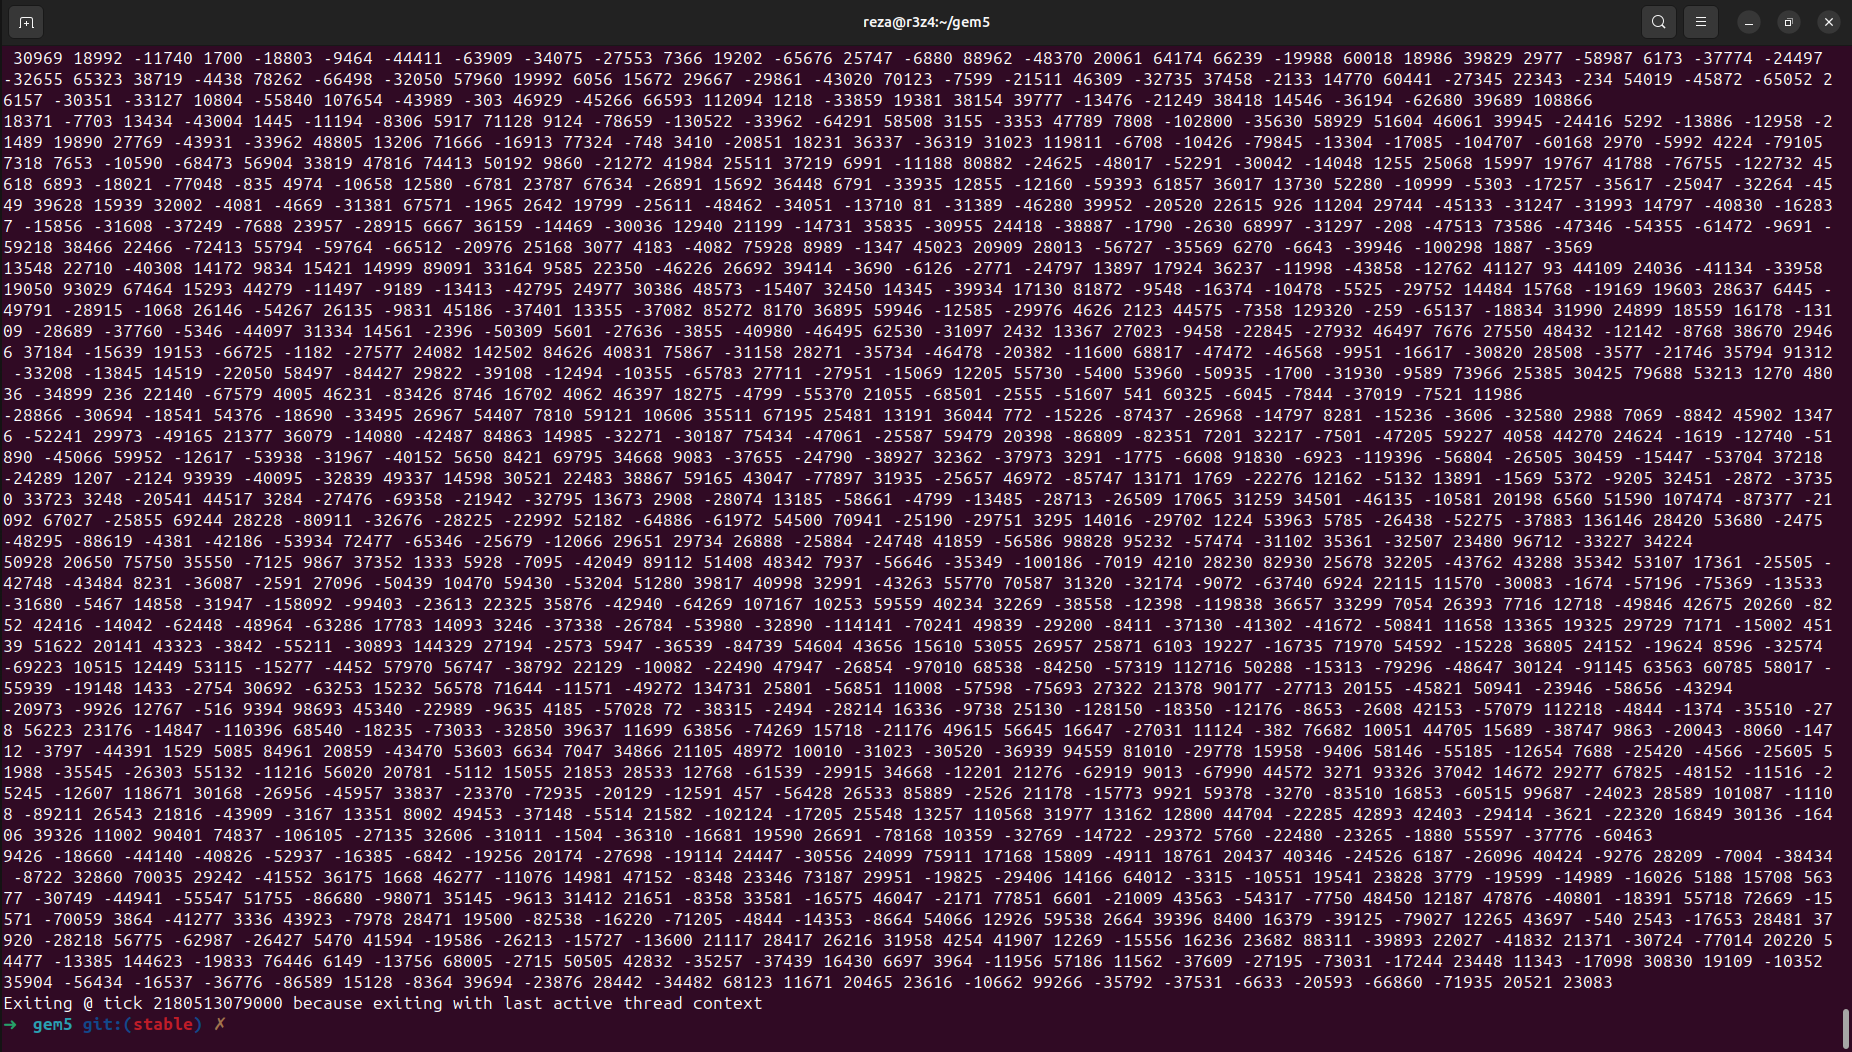
\includegraphics[scale=0.12]{images/img10.png}
			\caption{خروجی شبیه‌سازی شبه‌کد دوم}
			\label{خروجی شبیه‌سازی شبه‌کد دوم}
		\end{figure}
	\end{center}
	
	
	
	\subsection{گام چهارم}
	\subsubsection{شبه‌کد اول}
	
	\begin{latin}
		\begin{itemize}
			\item IPC = 0.263273 $\frac{count}{cycle}$
			\item Number of busy cycles: 1626196851.999000
			\item L1i cache hit rate: not found
			\item L1i cache miss rate: not found
			\item l1d cache hit rate: not found
			\item l1d cache miss rate: not found
			\item l2i cache hit rate: 169
			\item l2d cache hit rate: 26420
			\item l2i cache miss rate: 2129
			\item l2d cache miss rate: 14245
		\end{itemize}
	\end{latin}
	
	
	
	\subsubsection{شبه‌کد دوم}
	\begin{latin}
		\begin{itemize}
			\item IPC = 0.266907 $\frac{count}{cycle}$
			\item Number of busy cycles: 2180513078.999000
			\item L1i cache hit rate: not found
			\item L1i cache miss rate: not found
			\item l1d cache hit rate: not found
			\item l1d cache miss rate: not found
			\item l2i cache hit rate: 154
			\item l2d cache hit rate: 20844
			\item l2i cache miss rate: 0.932692
			\item l2d cache miss rate: 0.405934
		\end{itemize}
	\end{latin}
	
	
	\subsection{گام پنجم}
	در هر دو شبه‌کد از یک تابع تولید اعداد تصادفی استفاده شده است. و ماتریس‌های بکار رفته در هر دو کد یمسان است.
	
	در شبه‌کد اول صرفا هر سطر را در ستون ماتریس متناظرش ظرب کرده و حاصل ضرب هر درایه را با مقدار قبلی خودش جمع میکنیم. اما در شبه‌کد دوم، الگوریتم نوشته شده برای ضرب دو ماتریس بسیار پیچیده‌تر از الگوریتم اول است.
	
	می‌دانیم که بار محاسباتی حلقه های تو در تو برای سخت افزار بسیار سنگین است و تاجایی که ممکن است باید از نوشتن حلقه‌های تو در تو غیر ضروری پرهیز کنیم. پس می‌توان یکی از معیار‌های مقایسه این دو شبه‌کد را حلقه‌های تو در تو قرار داد.
	
	در شبه‌کد اول از ۳ حلقه \texttt{for} تو در تو استفاده شده است اما در شبه‌کد دوم از ۶ حلقه استفاده شده است. بنابر این می‌توان گفت که شبه‌کد دوم از نظر Performance کند تر و بار محاسباتی بیشتری را بر سیستم متحمل می‌شود و در بهترین حالت (با فرض برابر بودن باقی قسمت‌های کد) انتظار داریم شبه‌کد دوم حداقل ۲ برابر کند‌تر از شبه‌کد اول باشد.
	
	
	یکی از پارامتر‌های مقایسه \texttt{performance} دو پردازنده، \texttt{Cycle Per Instruction}
	یا با اختصار \texttt{IPC} است.
	این پارامتر، نشان دهنده میانگین \texttt{instruction} های انجام شده توسط \texttt{cpu} در هر کلاک است.
	
	پارامتر دیگری که برای مقایسه \texttt{performance} مورد استفاده قرار می‌گیرد، \texttt{Instruction Per Clock} یا همان \texttt{CPI} است. این پارامتر تعداد کلاک های زده شده برای انجام هر \texttt{instruction} را نشان می‌دهد.
	
	\texttt{CPI} و \texttt{IPC} دقیقا عکس هم هستند. برای مقایسه \texttt{performance} این دو شبه کد از پارامتر \texttt{CPI} استفاده می‌کنیم.
	
	در فایل \texttt{stats} شبه‌کد اول، \textbf{CPI=89.59} گزارش شده است.
	همچنین در شبه‌کد دوم، \textbf{CPI=101.82} است. همانطور که مشاهده می‌شود در شبه‌کد دوم، بار محاسباتی بیشتر بوده است و برای هر \texttt{instruction} به‌طور میانگین ۱۰۱ لبه کلاک مصرف شده است. که این تحلیل با نکته ای که در مورد حلقه‌های تو در تو در ابتدای این بخش گفتیم مطابقت دارد.
	
	پارامتر بعدی ای که می‌توان برای مقایسه \texttt{performance} دو کد استفاده کرد، \texttt{Clock Busy of Number} است. که نشان دهنده تعداد کلاک‌هایی است که \texttt{cpu} مشغول اجرای برنامه بوده است. شاید نتوان از این پارامتر برای مقایسه هر نوع برنامه ای استفاده کرد چون ممکن است معیار مناسبی برای مقیسه دو برنامه متفاوت نباشد، اما در اینجا چون ورودی‌ها و خروجی‌های هر دو برنامه یکسان است و فقط الگوریتم‌ها تفاوت دارد، معیار خوبی برای مقایسه \texttt{performance} است.
	
	این پارامتر برای شبه کد اول، 38357398549 و برای شبه‌کد دوم، 59261119215 بدست‌امده است. همانطور که مشاهده می‌شود، در این معیار هم بازنده \texttt{performance} شبه‌کد دوم است و اجرای شبه‌کد اول در تعداد کلاک های کمتری طول کشیده است. این خروجی هم مطابق با پیش‌بینی ای است که در ابتدا کرده بودیم.
	
	
	
	
	
	
	
	
	
	
	
	
	
	
	
	
	\section{پاسخ سوال دوم}
	مطابق با دستور زیر، فایل را در دو حالت AtomicSimpleCPU و DerivO3CPU شبیه‌سازی می‌کنیم:
	\begin{latin}
		\texttt{build/X86/gem5.opt configs/example/}
		\texttt{se.py ../../../Downloads/sample}
	\end{latin}
	
	\subsection{گام اول}
	
	پارامتر‌های IPC و Sim\_second برای حالت AtomicSimpleCPU به‌صورت زیر بدست آمده است:
	\begin{latin}
		\begin{enumerate}
			\item IPC = 0.262431 $\frac{count}{cycle}$
			\item Sim\_second: 20.413799
		\end{enumerate} 
	\end{latin}
	
	پارامتر‌های IPC و Sim\_second برای حالت DerivO3CPU به‌صورت زیر بدست آمده است:
	\begin{latin}
		\begin{enumerate}
			\item IPC: 0.278193 $\frac{count}{cycle}$
			\item Sim\_second: 38.17364
		\end{enumerate} 
	\end{latin}
	
	تفاوت اصلی بین حالت های AtomicSimpleCPU و DerivO3CPU در سطح جزئیات و پیچیدگی آنها در مدل سازی CPU نهفته است. برای مثال این یک نمایش اولیه از پایپ‌لاین CPU را بدون ویژگی های ریزمعماری دقیق ارائه می دهد. همچنین Instruction ها به صورت اتمی اجرا می شوند، به این معنی که در یک کلاک بدون در نظر گرفتن مراحل پایپ‌لاین یا تأخیرها کامل می شوند. AtomicSimpleCPU از نظر سرعت شبیه سازی سریعتر است اما دقت کمتری نسبت به DerivO3CPU دارد. به دلیل سادگی، AtomicSimpleCPU به طور کلی IPC و مقدار sim\_second کمتری نسبت به DerivO3CPU دارد. که همین موضوع از نتایج بدست آمده از شبیه‌سازی هم مشهود است.
	
	
	
	
	
	
	
	\subsection{گام دوم}
	برای افزایش سرعت دسترسی به حافظه می‌توان به جای تخصیص حافظه برای هر گره به صورت مجزا، با استفاده از \texttt{malloc} یک بلوک پیوسته از حافظه را برای همه گره‌ها به صورت همزمان اختصاص داد.
	
 انجام عملیات بازگشتی بازگشتی بار محاسباتی سنگینی را به \texttt{CPU} تحمیل می‌کند. می‌توان این اجرای بازگشتی را با یک تابع \texttt{iterative} جایگزین کرد.
 
 کد اصلاح شده را می‌توانید در «\textcolor{blue}{پیوست آ}» مشاهده کنید
	
	
	
	
	
	
	
	
	
	\section{پاسخ سوال سوم}
	برای شبیه‌سازی حافظه‌ها در \texttt{gem5} سه \texttt{mode} کاری وجود دارد. \texttt{mode Timing} و \texttt{mode Atomic} و \texttt{mode Functional} که در ادامه به بررسی تفاوت‌های آنها می‌پردازیم.

	\begin{enumerate}
		
		\item \textbf{mode :Functional }
		\begin{enumerate}
			\item این حالت، ساده ترین و سریع‌ترین حالت است.
			\item به دلیل اینکه این حالت ساده‌ترین حالت است و بسیاری از آپشن‌های حالات دیگر را ندارد، سرعت بیشتری هم دارد.
			\item این حالت برای شبیه‌سازی اولیه مناسب است.
			\item در این حالت، همه دسترسی‌های حافظه به‌صورت دقیق مدل نمی‌شود.
			‌\item بین دقت و سرعت، trade-off وجود دارد. بنابر این نمی‌توان از این حالت انتظار دقت بسیار بالایی داشت.
		\end{enumerate}
		
		
		\item \textbf{mode :Atomic }
		\begin{enumerate}
			\item این حالت سطح بالا‌تری ازجزئیات را در مقایسه با حالت functional ارائه می‌دهد.
			\item در این حالت تمام دسترسی‌های حافظه بدون درنظر گرفتن ملاحظات زمانی مدل می‌شوند.
			\item این حالت، سریع‌تر از حالت timing است و دقت بیشتری نسبت به حالت functional دارد.
		\end{enumerate}
		
		
		
		
		
		\item \textbf{mode :Timing }
		\begin{enumerate}
			\item دقیق‌ترین و جزءی ترین شبیه‌سازی را این حالت انجام می‌دهد.
			\item در این حالت بر خلاف حالت قبل، دسترسی‌ها به حافظه با ملاحظات و در نظر گرفتن زمان‌بندی ها و تاخیر‌ها مدل‌سازی می‌شود.
			\item این حالت از شبیه‌سازی رفتاری واقع گرایانه از سلسله‌مراتب کش، کنترل‌کننده های حافظه و تاخیر‌های اتصال را شبیه‌سازی می‌کند.
			\item این حالت بیشتر در ارزیابی و تاثیر بهینه‌سازی های مرتبط با حافظه استفاده می‌شود.
			\item این حالت از شبیه‌سازی دقیق‌ترین نتایج را ارائه می‌دهد اما در مقایسه با دو حالت قبل، به دلیل حجم محاسبات و شبیه‌سازی بیشتر، زمان‌ شبیه‌سازی بیشتر استو	
		\end{enumerate}
		
	\end{enumerate}
	
	انتخاب mode حافظه به نیازهای خاص شبیه سازی ما بستگی دارد. اگر به نتایج سریع و تقریبی نیاز داشته باشیم، می‌توان از حالت functional استفاده کرد. اما اگر به ویژگی های مرتب سازی حافظه اولیه نیاز داشته باشیم، می توان از حالت atomic استفاده کرد. برای تجزیه و تحلیل دقیق عملکرد و مطالعات ریزمعماری، حالت timing بهترین انتخاب برای شبیه‌سازی است.
	
	
	
	
	با بررسی فایل \texttt{config} گام اول سوال اول پارامتر های خواسته شده را به صورت زیر گزارش می‌کنیم:
	
	\textbf{فرکانس کلاک: } ۱ گیگا‌هرتز است.
	
	\begin{center}
		\begin{figure}[H]
			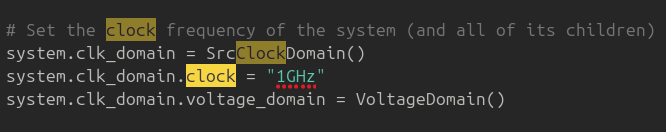
\includegraphics[scale=0.36]{images/img13.png}
			\caption{فرکانس کلاک شبیه‌سازی}
			\label{فرکانس کلاک}
		\end{figure}
	\end{center}
	
	\textbf{مد شبیه‌سازی: }مد شبیه‌سازی روی mode Timing تنظیم شده است.
	\begin{center}
		\begin{figure}[H]
			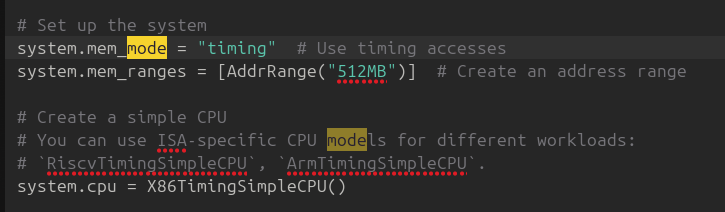
\includegraphics[scale=0.33]{images/img11.png}
			\caption{مد شبیه‌سازی}
			\label{مد شبیه‌سازی}
		\end{figure}
	\end{center}
	
	\textbf{سایز حافظه: }سایز حافظه ۵۱۲ مگابایت تعریف شده است.
	\begin{center}
		\begin{figure}[H]
			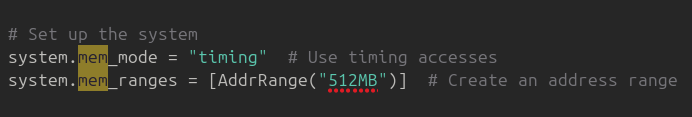
\includegraphics[scale=0.35]{images/img12.png}
			\caption{سایز حافظه}
			\label{سایز حافظه}
		\end{figure}
	\end{center}
	
	
	
	
	

		
\end{multicols}









\newpage
\fontsize{30}{30} \textbf{پیوست آ\label{پیوست آ}} \\ \\ \\

• کد پایتون نوشته شده برای شبه‌کد اول:
\begin{latin}
	\lstinputlisting[
	caption=Python code for part1,
	label={lst:listing-cpp},
	language=python,
	style=myStyle,
	]{codes/ACA_HW02_Part1.py}
\end{latin}





• کد C++ نوشته شده برای شبه‌کد اول:
\begin{latin}
	\lstinputlisting[
	caption=C++ code for part1,
	label={lst:listing-cpp},
	language=C++,
	style=myStyle,
	]{codes/ACA_HW02_Part1.cpp}
\end{latin}







• کد پایتون نوشته شده برای شبه‌کد دوم:
\begin{latin}
	\lstinputlisting[
	caption=Python code for part2,
	label={lst:listing-cpp},
	language=python,
	style=myStyle,
	]{codes/ACA_HW02_Part2.py}
\end{latin}






• کد C++ نوشته شده برای شبه‌کد دوم:
\begin{latin}
	\lstinputlisting[
	caption=C++ code for part2,
	label={lst:listing-cpp},
	language=C++,
	style=myStyle,
	]{codes/ACA_HW02_Part2.cpp}
\end{latin}


• کد موجود در فایل Sample.c: 
\begin{latin}
	\lstinputlisting[
	caption=Sample C code,
	label={lst:listing-cpp},
	language=C++,
	style=myStyle,
	]{codes/sample.c}
\end{latin}




• کد Sample.c بهبود داده شده:
\begin{latin}
	\lstinputlisting[
	caption=Improved C code,
	label={lst:listing-cpp},
	language=C++,
	style=myStyle,
	]{codes/sample_Improved.c}
\end{latin}




\end{document}